% !TEX root = task-3-3-2.tex
% Editable task bank. Append new BankTask blocks at the end of the document.
\documentclass[12pt,a4paper]{article}
\usepackage{physics-textbook}
\usepackage{graphicx,needspace}
\usetikzlibrary{decorations.pathmorphing}
\newif\ifShowSolutions
\ifdefined\TutorEdition
  \ShowSolutionstrue
\else
  \ShowSolutionsfalse % Change to \ShowSolutionstrue to display solutions.
\fi
\newcounter{banktask}
\newsavebox{\BankTaskBox}
\newcommand{\BankTaskContent}[3]{%
  \noindent\textbf{\thebanktask.}\quad #2\par
  \ifShowSolutions
    \Needspace{50mm}% Keep the solution heading with its opening text or diagram.
    #3\par
    \ifdefined\TutorEdition
      \ifcsname TutorSource#1\endcsname
        \nopagebreak\smallskip{\small\csname TutorSource#1\endcsname\par}%
      \fi
    \fi
  \fi
}
\newcommand{\BankTask}[3]{%
  \refstepcounter{banktask}\par\medskip
  \sbox{\BankTaskBox}{\begin{minipage}{\linewidth}%
    \BankTaskContent{#1}{#2}{#3}\end{minipage}}%
  \ifdim\dimexpr\ht\BankTaskBox+\dp\BankTaskBox\relax>\dimexpr\textheight-20mm\relax
    \Needspace{35mm}\BankTaskContent{#1}{#2}{#3}%
  \else
    \Needspace{\dimexpr\ht\BankTaskBox+\dp\BankTaskBox\relax}%
    \noindent\usebox{\BankTaskBox}\par
  \fi
  \medskip
}
\begin{document}
\BookSubsection{3.3.2}{Электрическое поле}


% Source DDF127: https://ege.fipi.ru/bank/questions.php?search=1&proj=BA1F39653304A5B041B656915DC36B38&qid=DDF127
\BankTask{DDF127}{
В первой экспериментальной установке положительно заряженная частица влетает в однородное электрическое поле так, что вектор $\vec{\upsilon}_0$ перпендикулярен вектору напряжённости электрического поля $\vec{E}$ (рис. 1). Во второй экспериментальной установке вектор $\vec{\upsilon}_0$ такой же частицы параллелен вектору индукции магнитного поля $\vec{B}$ (рис. 2).

По каким траекториям движутся частицы в этих установках? Силу тяжести не учитывать.

\TaskMatchingColumns[0.47\linewidth]{Движение частицы}{
А) в первой установке\par
Б) во второй установке
}{Траектория}{
1) прямая линия\par
2) окружность\par
3) спираль\par
4) парабола
}

\begin{center}
\begin{tabular}{|c|c|}
\hline
А & Б \\
\hline
\phantom{0} & \phantom{0} \\
\hline
\end{tabular}
\end{center}

\begin{center}
\begin{tikzpicture}[book diagram,line cap=round,line join=round]
\begin{scope}[x=0.65cm,y=0.65cm]
\foreach \x in {0,1,2,3,4,5}{
  \foreach \y in {0,1,2,3,4,5}{
    \draw (\x,\y) circle[radius=0.20];
    \fill (\x,\y) circle[radius=0.035];
  }
}
\draw[fill=white] (3.37,2.52) circle[radius=0.23];
\node at (3.37,2.52) {$+$};
\draw[-{book tip}] (2.33,2.52)--(3.03,2.52);
\node[above] at (2.67,2.59) {$\vec{\upsilon}_0$};
\node at (5.58,3.55) {$\vec E$};
\node at (2.5,-0.65) {Рис. 1};
\end{scope}
\begin{scope}[shift={(5.4cm,0cm)},x=0.65cm,y=0.65cm]
\foreach \x in {0,1.2,2.4}{
  \draw[-{book tip}] (\x,0.4)--(\x,4.75);
}
\draw[fill=white] (0.45,2.75) circle[radius=0.23];
\node at (0.45,2.75) {$+$};
\draw[-{book tip}] (0.45,2.46)--(0.45,1.78);
\node[right] at (0.48,2.03) {$\vec{\upsilon}_0$};
\node[right] at (2.45,4.75) {$\vec B$};
\node at (1.2,-0.65) {Рис. 2};
\end{scope}
\end{tikzpicture}
\end{center}
}{
\smallskip\noindent\textbf{Решение от GPT}\par
В первой установке постоянная сила $\vec F=q\vec E$ сообщает частице ускорение, перпендикулярное начальной скорости: $x=\upsilon_0t$, $z=qEt^2/(2m)$, поэтому траектория --- парабола (4). Во второй установке $\vec\upsilon_0$ антипараллелен $\vec B$, как показано на рисунке, поэтому $F_{\text{Л}}=q\upsilon B\sin180^\circ=0$ и частица движется по прямой (1). Окружность (2) требует поперечной магнитной силы, а спираль (3) --- одновременно ненулевых продольной и поперечной составляющих скорости в магнитном поле; здесь этих условий нет. Ответ: А --- 4, Б --- 1.
}

% Source AE92AD: https://ege.fipi.ru/bank/questions.php?search=1&proj=BA1F39653304A5B041B656915DC36B38&qid=AE92AD
\BankTask{AE92AD}{
В первой экспериментальной установке положительно заряженная частица влетает в однородное электрическое поле так, что вектор скорости $\vec{\upsilon}_0$ частицы параллелен вектору напряжённости электрического поля $\vec{E}$ (рис. 1). Во второй установке вектор скорости $\vec{\upsilon}_0$ отрицательно заряженной частицы перпендикулярен вектору индукции магнитного поля $\vec{B}$ (рис. 2).

По каким траекториям движутся частицы в этих установках? Силой тяжести пренебречь.

\TaskMatchingColumns[0.47\linewidth]{Движение частицы}{
А) в первой установке\par
Б) во второй установке
}{Траектория}{
1) прямая линия\par
2) окружность\par
3) спираль\par
4) парабола
}

\begin{center}
\begin{tabular}{|c|c|}
\hline
А & Б \\
\hline
\phantom{0} & \phantom{0} \\
\hline
\end{tabular}
\end{center}

\begin{center}
\begin{tikzpicture}[book diagram,line cap=round,line join=round]
\begin{scope}[x=0.70cm,y=0.70cm]
\foreach \x in {0,1.2,2.4}{
  \draw[-{book tip}] (\x,4.4)--(\x,0);
}
\draw[fill=white] (0.45,2.35) circle[radius=0.23];
\node at (0.45,2.35) {$+$};
\draw[-{book tip}] (0.45,2.64)--(0.45,3.30);
\node[right] at (0.47,3.05) {$\vec{\upsilon}_0$};
\node[right] at (2.45,4.35) {$\vec E$};
\node at (1.2,-0.65) {Рис. 1};
\end{scope}
\begin{scope}[shift={(4.5cm,0.45cm)},x=0.70cm,y=0.70cm]
\foreach \x in {0,1.6,3.2}{
  \foreach \y in {0,1.6,3.2}{
    \draw (\x-0.25,\y-0.25)--(\x+0.25,\y+0.25);
    \draw (\x-0.25,\y+0.25)--(\x+0.25,\y-0.25);
  }
}
\draw[fill=white] (1.10,2.40) circle[radius=0.30];
\node at (1.10,2.40) {$-$};
\draw[-{book tip}] (1.43,2.40)--(3.05,2.40);
\node[above] at (2.30,2.50) {$\vec{\upsilon}_0$};
\node[right] at (3.45,0.80) {$\vec B$};
\node at (1.6,-1.29) {Рис. 2};
\end{scope}
\end{tikzpicture}
\end{center}
}{
\smallskip\noindent\textbf{Решение от GPT}\par
В первой установке сила $\vec F=q\vec E$ направлена вдоль той же прямой, что и начальная скорость, поэтому траектория --- прямая (1), в том числе после возможной остановки и движения обратно. Во второй установке сила Лоренца перпендикулярна скорости и служит центростремительной: $|q|\upsilon B=m\upsilon^2/r$, поэтому траектория --- окружность (2). Спирали (3) нет, поскольку отсутствует составляющая скорости вдоль магнитного поля; параболы (4) нет, поскольку в первой установке отсутствует начальная поперечная скорость. Ответ: А --- 1, Б --- 2.
}

% Source 43028: https://phys-ege.sdamgia.ru/problem?id=43028
\BankTask{43028}{
В вакууме в однородное горизонтальное электрическое поле с напряженностью E  =  $1000$ кВ/м помещают неподвижную капельку массой m  =  $0{,}4\,\text{г}$ и зарядом q  =  $3\,\text{нКл}$. Определите скорость капельки через t  =  $0{,}2\,\text{с}$. Сделайте рисунок, на котором укажите силы, действующие на капельку.
}{
\smallskip\noindent\textbf{Решение}\par
\begin{center}\begin{tikzpicture}[>=stealth]

\draw[->](-.65,1.05)--(2.55,1.05)node[midway,above]{$\vec E$};
\fill (0,.38) circle(.055);\draw[->](0,.38)--(1.25,.38) node[right]{$\vec F_{\!\text{э}}$};\draw[->](0,.38)--(0,-.65)node[below]{$m\vec g$};
\end{tikzpicture}\end{center}
На капельку действуют сила тяжести $m \vec{g}$ и сила действия электрического поля, направленная по линиям напряженности и равная $F_{\,\text{э}}=Eq.$
Равнодействующая этих сил постоянна и по второму закону Ньютона равна 

\[m \vec{g} + \vec F_{\,\text{э}}=m \vec{a} .\]

По горизонтальной оси: проекция ускорения капельки

\[a_x= \frac{Eq}{m} ,\]

тогда проекция скорости на горизонтальную ось при равноускоренном движении без начальной скорости

\[v _x= a_xt= \frac{Eqt}{m} .\]

По вертикали под действием силы тяжести $a_y=g,$ поэтому вертикальная проекция скорости капельки равна 

\[v _y=gt.\]

Тогда скорость капли через промежуток времени t равна

\[v = \sqrt{v _x ^2 + v _y ^2} =t \sqrt{( \frac{Eq}{m} ) ^2 + g ^2} =0{,}2 \cdot \sqrt{( \frac{3 \cdot 10^{-9} \cdot 10^{6}}{4 \cdot 10 ^{ - 4 }} ) ^2 + 100} =2{,}5 \,\text{м/с} .\]

Ответ: $2{,}5\,\text{м/с}$.
}

% Source 30002: https://phys-ege.sdamgia.ru/problem?id=30002
\BankTask{30002}{
\begin{center}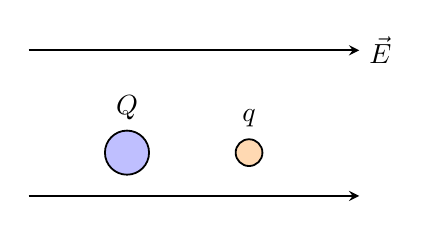
\begin{tikzpicture}[>=stealth,line width=.65pt]\draw[->](0,1.3)--(4.2,1.3)node[right]{$\vec E$};\draw[->](0,-.55)--(4.2,-.55);\draw[fill=blue!25](1.25,0)circle(.28)node[above=.29cm]{$Q$};\draw[fill=orange!30](2.8,0)circle(.17)node[above=.2cm]{$q$};\end{tikzpicture}\end{center}

В однородном электрическом поле с напряженностью E  =  $18\,\text{В}$/м находятся два точечных заряда: Q  =  -$1\,\text{нКл}$ и $q= + 5$ нКл с массами M  =  $5\,\text{г}$ и m  =  $10\,\text{г}$ соответственно (см. рисунок). На каком расстоянии d друг от друга находятся заряды, если их ускорения совпадают по величине и направлению? Сделайте рисунок с указанием всех сил, действующих на заряды. Силой тяжести пренебречь.
}{
\smallskip\noindent\textbf{Решение}\par
\begin{center}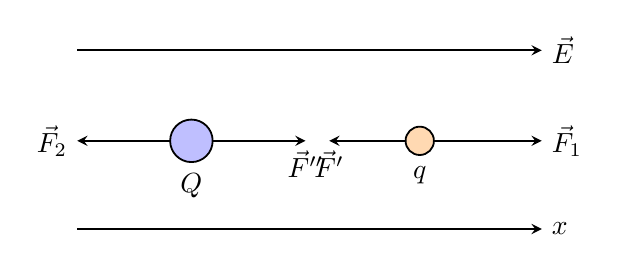
\begin{tikzpicture}[>=stealth,line width=.65pt]\draw[->](0,1.15)--(5.9,1.15)node[right]{$\vec E$};\draw[->](0,-1.12)--(5.9,-1.12)node[right]{$x$};\draw[fill=blue!25](1.45,0)circle(.27)node[below=.29cm]{$Q$};\draw[fill=orange!30](4.35,0)circle(.18)node[below=.2cm]{$q$};\draw[->](1.18,0)--(0,0)node[left]{$\vec F_2$};\draw[->](1.72,0)--(2.9,0)node[below]{$\vec F^{\prime\prime}$};\draw[->](4.17,0)--(3.2,0)node[below]{$\vec F^{\prime}$};\draw[->](4.53,0)--(5.9,0)node[right]{$\vec F_1$};\end{tikzpicture}\end{center}

$1$.  Направим ось Ox по напряженности электрического поля $\vec{E}.$ На заряд q действуют две электрические силы: $F_1=q E$ со стороны однородного поля и сила Кулона $F ^{ \prime } =F= \frac{k q|Q|}{d ^2}$ со стороны другого заряда. На заряд Q действуют сила $F_2=|Q| E$ со стороны однородного поля и сила Кулона $F ^{ \prime \prime } =F= \frac{k q|Q|}{d ^2}$ со стороны заряда q. 
$2$.  В соответствии со вторым законом Ньютона в проекциях на ось Ox имеем: 

$m a=F_1 - F, \qquad ( 1 )$ $M a= - F_2 + F.\qquad ( 2 )$

 Тогда из соотношений ($1$) и ($2$) и условия задачи получим: 

\[\frac{F_1 - F}{m} = \frac{F - F_2}{M} . \qquad ( 3 )\]

$3$.  Подставляя в ($3$) выражения для электрических сил, получим: 

\[d=\sqrt{\frac{kq|Q|(m+M)}{E(m|Q|+qM)}}=\sqrt{\frac{9\cdot10^9\cdot5\cdot10^{-9}\cdot1\cdot10^{-9}\cdot(0{,}01+0{,}005)}{18(0{,}01\cdot1\cdot10^{-9}+0{,}005\cdot5\cdot10^{-9})}}\approx1\,\text{м}.\]

Ответ: $d \approx 1 \,\text{м}.$
}

\end{document}
